% --- INSTITUTIONAL TEMPLATE FED v7.4.9 ---
% Estándar de Reporteo APA 7 (Babel-Free)
\documentclass[12pt,spanish]{article}

\usepackage{graphicx}
\usepackage{geometry}
\usepackage{indentfirst} 
\usepackage{caption}
\usepackage{floatrow} 

% Forzar estilos de caption antes de cualquier carga
\floatsetup[figure]{capposition=top}
\floatsetup[table]{capposition=top}

\usepackage{booktabs}
\usepackage{float}
\usepackage{longtable}
\usepackage{threeparttable}
\usepackage{array}
\usepackage{calc}
\usepackage{amsmath, amssymb}
\usepackage{fancyhdr}
\usepackage{mathptmx} 
\usepackage[T1]{fontenc}
\usepackage{setspace} 
\usepackage{ragged2e} 
\usepackage{titlesec}
\usepackage{url}
\def\UrlBreaks{\do\/\do-\do\.\do\_\do\?\do\=\do\&\do\%}
\usepackage[hidelinks,breaklinks]{hyperref}
\usepackage{xcolor}
\usepackage{fancyvrb}
\usepackage{framed}

% --- Code Highlighting (Pandoc Standard) ---
\newenvironment{Shaded}{\begin{snugshade}}{\end{snugshade}}
\definecolor{shadecolor}{RGB}{248,248,248}
\newenvironment{Highlighting}{}{}
\newcommand{\VerbBar}{|}
\newcommand{\VERB}{\Verb[commandchars=\\\{\}]}
\DefineVerbatimEnvironment{Highlighting}{Verbatim}{commandchars=\\\{\}}
\newcommand{\AlertTok}[1]{\textcolor[rgb]{0.94,0.16,0.16}{#1}}
\newcommand{\AnnotationTok}[1]{\textcolor[rgb]{0.56,0.35,0.01}{\textbf{\textit{#1}}}}
\newcommand{\AttributeTok}[1]{\textcolor[rgb]{0.13,0.29,0.53}{#1}}
\newcommand{\BaseNTok}[1]{\textcolor[rgb]{0.00,0.00,0.81}{#1}}
\newcommand{\BuiltInTok}[1]{#1}
\newcommand{\CharTok}[1]{\textcolor[rgb]{0.31,0.60,0.02}{#1}}
\newcommand{\CommentTok}[1]{\textcolor[rgb]{0.56,0.35,0.01}{\textit{#1}}}
\newcommand{\CommentVarTok}[1]{\textcolor[rgb]{0.56,0.35,0.01}{\textbf{\textit{#1}}}}
\newcommand{\ConstantTok}[1]{\textcolor[rgb]{0.56,0.35,0.01}{#1}}
\newcommand{\ControlFlowTok}[1]{\textcolor[rgb]{0.13,0.29,0.53}{\textbf{#1}}}
\newcommand{\DataTypeTok}[1]{\textcolor[rgb]{0.13,0.29,0.53}{#1}}
\newcommand{\DecValTok}[1]{\textcolor[rgb]{0.00,0.00,0.81}{#1}}
\newcommand{\DocumentationTok}[1]{\textcolor[rgb]{0.56,0.35,0.01}{\textbf{\textit{#1}}}}
\newcommand{\ErrorTok}[1]{\textcolor[rgb]{0.64,0.00,0.00}{\textbf{#1}}}
\newcommand{\ExtensionTok}[1]{#1}
\newcommand{\FloatTok}[1]{\textcolor[rgb]{0.00,0.00,0.81}{#1}}
\newcommand{\FunctionTok}[1]{\textcolor[rgb]{0.13,0.29,0.53}{\textbf{#1}}}
\newcommand{\ImportTok}[1]{#1}
\newcommand{\InformationTok}[1]{\textcolor[rgb]{0.56,0.35,0.01}{\textbf{\textit{#1}}}}
\newcommand{\KeywordTok}[1]{\textcolor[rgb]{0.13,0.29,0.53}{\textbf{#1}}}
\newcommand{\NormalTok}[1]{#1}
\newcommand{\OperatorTok}[1]{\textcolor[rgb]{0.81,0.36,0.00}{\textbf{#1}}}
\newcommand{\OtherTok}[1]{\textcolor[rgb]{0.56,0.35,0.01}{#1}}
\newcommand{\PreprocessorTok}[1]{\textcolor[rgb]{0.56,0.35,0.01}{\textit{#1}}}
\newcommand{\RegionMarkerTok}[1]{#1}
\newcommand{\SpecialCharTok}[1]{\textcolor[rgb]{0.81,0.36,0.00}{\textbf{#1}}}
\newcommand{\SpecialStringTok}[1]{\textcolor[rgb]{0.31,0.60,0.02}{#1}}
\newcommand{\StringTok}[1]{\textcolor[rgb]{0.31,0.60,0.02}{#1}}
\newcommand{\VariableTok}[1]{\textcolor[rgb]{0.00,0.00,0.00}{#1}}
\newcommand{\VerbatimStringTok}[1]{\textcolor[rgb]{0.31,0.60,0.02}{#1}}
\newcommand{\WarningTok}[1]{\textcolor[rgb]{0.56,0.35,0.01}{\textbf{\textit{#1}}}}

% --- Pandoc Compatibility Block (Iron Clad) ---
\providecommand{\tightlist}{%
  \setlength{\itemsep}{0pt}\setlength{\parskip}{0pt}}

% Compatibilidad Pandoc 3.x
\ifdefined\pandocbounded\else
  \newcommand{\pandocbounded}[1]{#1}
\fi

% --- Pandoc Citeproc (CSL) compatibility ---
\newlength{\cslhangindent}
\setlength{\cslhangindent}{1.27cm} 
\newlength{\csllabelwidth}
\setlength{\csllabelwidth}{3em}
\newcommand{\citeproctext}{} 
\newcommand{\citeprocitem}[2]{\item} 
\newenvironment{CSLReferences}[2] 
 {\begin{list}{}{
  \setlength{\leftmargin}{\cslhangindent}
  \setlength{\parsep}{0pt}
  \setlength{\itemsep}{6pt}
  \ifodd #1
   \setlength{\leftmargin}{\leftmargin + \csllabelwidth}
   \setlength{\itemindent}{-\csllabelwidth}
  \fi
  }
  \renewcommand{\bibitem}[2][]{\item} % Elimina los corchetes [ ]
 }
 {\end{list}}
\newcommand{\CSLBlock}[1]{#1\hfill\break}
\newcommand{\CSLLeftMargin}[1]{\parbox[t]{\csllabelwidth}{#1}}
\newcommand{\CSLRightInline}[1]{\parbox[t]{\linewidth - \csllabelwidth}{#1}\break}
\newcommand{\CSLIndent}[1]{\hspace{\cslhangindent}#1}

\makeatletter
\@ifundefined{paragraph}{\newcounter{paragraph}}{}
\@ifundefined{subparagraph}{\newcounter{subparagraph}}{}
\makeatother

% Solución al error 'No counter none defined' en longtable
\makeatletter
\newcounter{none}
\@ifpackageloaded{caption}{
  \DeclareCaptionType{none}
  \captionsetup[none]{name=Tabla}
}{}
\makeatother

\hypersetup{
  colorlinks=true,
  linkcolor=blue,
  filecolor=blue,
  citecolor=blue,
  urlcolor=blue
}

% --- Macros Institucionales ---
\newcommand{\fuente}[1]{
  \vspace{4pt}
  \begin{flushleft}
    \small
    \textit{Nota.} #1
  \end{flushleft}
}

% --- Localización Manual Determinista (Sin Babel) ---
\AtBeginDocument{
  \renewcommand{\tablename}{Tabla}
  \renewcommand{\figurename}{Figura}
  \renewcommand{\contentsname}{Índice}
  \renewcommand{\listtablename}{Índice de Tablas}
  \renewcommand{\listfigurename}{Índice de Figuras}
  \renewcommand{\abstractname}{Resumen}
  \renewcommand{\refname}{Referencias}
  
  \RaggedRight
  \setlength{\parindent}{1.27cm}
  \setlength{\parskip}{0pt}
}

\DeclareCaptionLabelSeparator{newline}{\\ \vspace{2pt}}
\captionsetup{
  position=top,
  justification=RaggedRight,
  singlelinecheck=false,
  labelfont=bf,
  textfont=it,
  labelsep=newline,
  font=small,
  skip=10pt
}
\captionsetup[figure]{name=Figura}
\captionsetup[table]{name=Tabla}

% Márgenes APA 7
\geometry{
  a4paper,
  margin=25.4mm,
  headheight=15mm
}

% --- Encabezados ---
\pagestyle{fancy}
\fancyhf{} 
\fancyhead[L]{
\includegraphics[height=1.2cm]{/home/erick-fcs/Capital_Workstation/capital-workstation-libs/src/ecs_quantitative/reporting/assets/logos/logo_unl.png}}
\fancyhead[R]{
\includegraphics[height=1.2cm]{/home/erick-fcs/Capital_Workstation/capital-workstation-libs/src/ecs_quantitative/reporting/assets/logos/logo_economia.jpg}}
\renewcommand{\headrulewidth}{0pt}
\fancyfoot[R]{\thepage}

\fancypagestyle{plain}{
  \fancyhf{}
  \fancyhead[L]{
\includegraphics[height=1.2cm]{/home/erick-fcs/Capital_Workstation/capital-workstation-libs/src/ecs_quantitative/reporting/assets/logos/logo_unl.png}}
  \fancyhead[R]{
\includegraphics[height=1.2cm]{/home/erick-fcs/Capital_Workstation/capital-workstation-libs/src/ecs_quantitative/reporting/assets/logos/logo_economia.jpg}}
  \fancyfoot[R]{\thepage}
  \renewcommand{\headrulewidth}{0pt}
}

% --- Títulos ---
\titleformat{\section}{\normalfont\normalsize\bfseries\centering}{\thesection}{1em}{}
\titleformat{\subsection}{\normalfont\normalsize\bfseries}{\thesubsection}{1em}{}
\titleformat{\subsubsection}{\normalfont\normalsize\bfseries\itshape}{\thesubsubsection}{1em}{}
\titlespacing*{\section}{0pt}{12pt}{6pt}
\titlespacing*{\subsection}{0pt}{12pt}{6pt}
\titlespacing*{\subsubsection}{0pt}{12pt}{6pt}

\newenvironment{referenciasAPA}{
  \setlength{\parindent}{-1.27cm}
  \setlength{\leftskip}{1.27cm}
  \setlength{\parskip}{6pt}
}{\par}

\begin{document}

\begin{center}
    {\bfseries \Large Universidad Nacional de Loja}\\[0.3cm]
    {\bfseries \large Facultad Jurídica, Social y
Administrativa}\\[0.2cm]
    {\bfseries Carrera de Economía}\\[1.5cm]
    
    {\bfseries \large Econometría Aplicada}\\[1cm]
    
    {\bfseries \Large ACD1-B: Evaluación de Impacto --- Educación
Superior y Formalidad}\\[1.5cm]
\end{center}

\noindent {\bfseries Estudiante:} Erick Fabricio Condoy Seraquive \\
\noindent {\bfseries Docente:} Eco. José Rafael Alvarado López \\
\noindent {\bfseries Fecha:} 20 de abril de 2026 \\

\vspace{1cm}

\doublespacing
\setlength{\parindent}{1.27cm}

\section{Introducción}\label{introducciuxf3n}

El presente estudio analiza los retornos a la educación en el mercado
laboral ecuatoriano bajo un enfoque de evaluación de impacto. Se busca
determinar si la obtención de un título de \textbf{Educación Superior}
actúa como un motor de formalización laboral y mejora salarial, aislando
el efecto del capital humano de otros factores sociodemográficos
(Shmueli 2010). Utilizando microdatos de la ENEMDU 2024, se compara a
individuos con educación superior frente a aquellos que solo alcanzaron
niveles inferiores, aplicando técnicas de emparejamiento para asegurar
la comparabilidad.

\section{Descripción de Variables}\label{descripciuxf3n-de-variables}

La base de datos se ha filtrado para incluir únicamente a la Población
Económicamente Activa (PEA) de entre 15 y 65 años con registros
completos de ingresos y sector de ocupación (INEC 2024).

\begin{longtable}[]{@{}
  >{\raggedright\arraybackslash}p{(\linewidth - 6\tabcolsep) * \real{0.2500}}
  >{\raggedright\arraybackslash}p{(\linewidth - 6\tabcolsep) * \real{0.2500}}
  >{\raggedright\arraybackslash}p{(\linewidth - 6\tabcolsep) * \real{0.2500}}
  >{\raggedright\arraybackslash}p{(\linewidth - 6\tabcolsep) * \real{0.2500}}@{}}
\caption{Variables para el análisis de impacto
educativo}\label{tbl-vars-edu}\tabularnewline
\toprule\noalign{}
\begin{minipage}[b]{\linewidth}\raggedright
Variable
\end{minipage} & \begin{minipage}[b]{\linewidth}\raggedright
Tipo
\end{minipage} & \begin{minipage}[b]{\linewidth}\raggedright
Descripción
\end{minipage} & \begin{minipage}[b]{\linewidth}\raggedright
Fuente
\end{minipage} \\
\midrule\noalign{}
\endfirsthead
\toprule\noalign{}
\begin{minipage}[b]{\linewidth}\raggedright
Variable
\end{minipage} & \begin{minipage}[b]{\linewidth}\raggedright
Tipo
\end{minipage} & \begin{minipage}[b]{\linewidth}\raggedright
Descripción
\end{minipage} & \begin{minipage}[b]{\linewidth}\raggedright
Fuente
\end{minipage} \\
\midrule\noalign{}
\endhead
\bottomrule\noalign{}
\endlastfoot
\texttt{age} & Entero & Edad cronológica (15-65 años) & ENEMDU \\
\texttt{sex} & Binaria & Género (1: Hombre; 0: Mujer) & ENEMDU \\
\texttt{hh\_size} & Entero & Número de miembros en el hogar & ENEMDU \\
\texttt{area} & Binaria & Sector de residencia (1: Urbana; 0: Rural) &
ENEMDU \\
\texttt{treated} & Binaria & Posee educación superior (Tratamiento) &
ENEMDU \\
\texttt{formal} & Binaria & Empleo en el sector formal (Variable de
Resultado 1) & ENEMDU \\
\texttt{income} & Continuo & Ingreso laboral mensual en USD (Variable de
Resultado 2) & ENEMDU \\
\end{longtable}

\section{Metodología}\label{metodologuxeda}

Se emplea el algoritmo de \textbf{Propensity Score Matching (PSM)} con
un modelo Logit para estimar la probabilidad de poseer educación
superior. El emparejamiento se realiza mediante el método del
\textbf{Vecino más Cercano (1:1)} con un \emph{caliper} de
\(0.25\sigma\). Se analizan dos indicadores de desempeño laboral: la
probabilidad de inserción formal y el nivel de ingresos.

\section{Resultados}\label{resultados}

\subsection{Efecto Medio del Tratamiento
(ATT)}\label{efecto-medio-del-tratamiento-att}

Los resultados confirman el alto valor del capital humano en el Ecuador.
Los individuos con educación superior, comparados con sus pares de
similar edad, sexo y ubicación geográfica, presentan:

\begin{enumerate}
\def\labelenumi{\arabic{enumi}.}
\tightlist
\item
  \textbf{Formalidad:} Un incremento de \textbf{21.50 puntos
  porcentuales} en la probabilidad de trabajar en el sector formal.
\item
  \textbf{Ingresos:} Una ganancia salarial mensual promedio de
  \textbf{\$313.63 USD}, lo que representa un retorno del
  \textbf{81.29\%} respecto al grupo de control.
\end{enumerate}

\subsection{Verificación de Soporte Común y
Balance}\label{verificaciuxf3n-de-soporte-comuxfan-y-balance}

La Figure~\ref{fig-pscore-edu} muestra una distribución de puntajes de
propensión con un traslape significativo, validando el supuesto de
soporte común. La Figure~\ref{fig-balance-edu} confirma que el
emparejamiento logró equilibrar la variable edad entre grupos.

\begin{figure}

\centering{

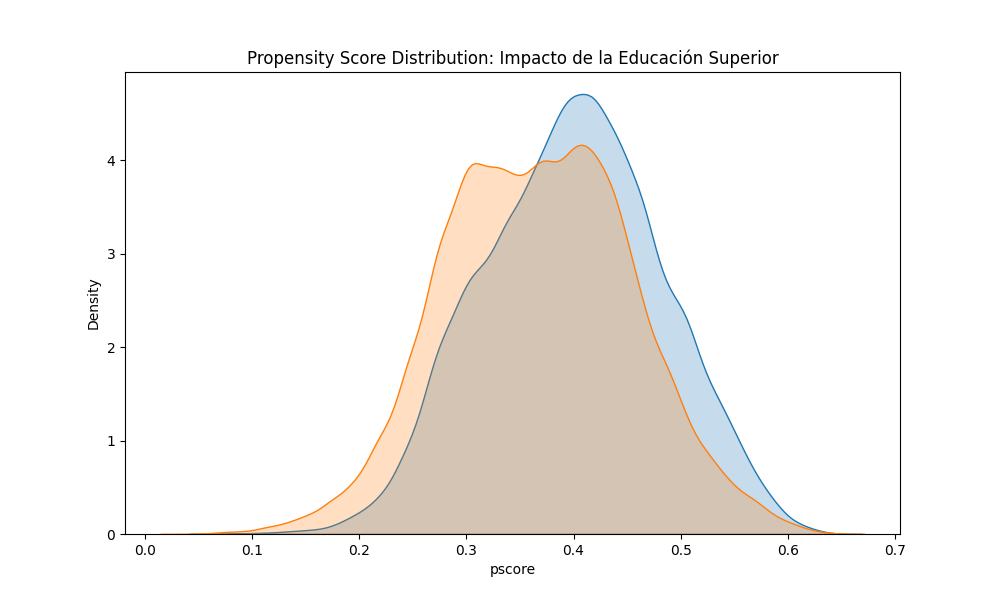
\includegraphics[width=0.75\linewidth,height=\textheight,keepaspectratio]{results_edu/common_support_edu.png}

}

\caption{\label{fig-pscore-edu}Distribución de Propensity Score:
Educación Superior}

\end{figure}%

\begin{figure}

\centering{

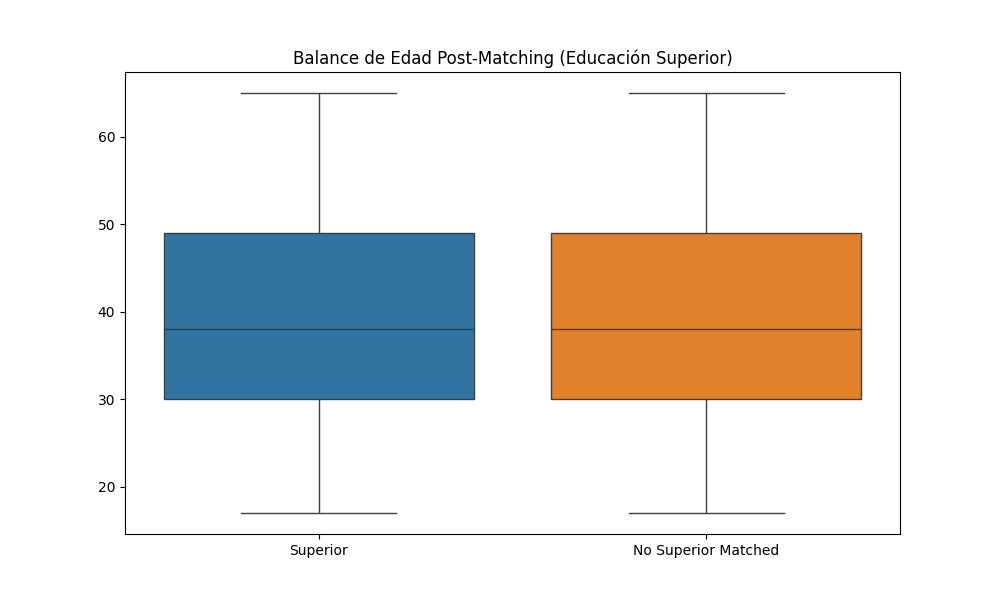
\includegraphics[width=0.75\linewidth,height=\textheight,keepaspectratio]{results_edu/age_balance_edu.png}

}

\caption{\label{fig-balance-edu}Balance de Covariables (Edad)
Post-Matching}

\end{figure}%

\section{Conclusión}\label{conclusiuxf3n}

La educación superior no solo mejora el flujo de ingresos directos
(efecto precio), sino que transforma la calidad del vínculo laboral
(efecto estructura) al triplicar prácticamente la probabilidad de acceso
a la seguridad social y la formalidad. Estos hallazgos subrayan la
importancia de las políticas de acceso a la universidad como mecanismos
eficaces de movilidad social y reducción de la precariedad laboral en
Ecuador.

\section{Referencias}\label{referencias}

\protect\phantomsection\label{refs}
\begin{CSLReferences}{1}{1}
\bibitem[\citeproctext]{ref-enemdu2024}
INEC. 2024. \emph{Encuesta Nacional de Empleo, Desempleo y Subempleo
(ENEMDU): Metodología de Cálculo de La Informalidad}. Instituto Nacional
de Estadística y Censos de Ecuador.

\bibitem[\citeproctext]{ref-shmueli2010}
Shmueli, Galit. 2010. {``To Explain or to Predict?''} \emph{Statistical
Science} 25 (3): 289--310.

\end{CSLReferences}

\end{document}
